\PassOptionsToPackage{hyphens}{url}
\documentclass[11pt,a4paper]{article}
\usepackage[T1]{fontenc}
\usepackage[utf8]{inputenc}
\usepackage[spanish,es-noquoting,es-tabla]{babel}
\usepackage{amsmath,amssymb}
\usepackage{booktabs}
\usepackage{graphicx}
\usepackage[margin=2.0cm,top=1.7cm,bottom=1.9cm]{geometry}
\usepackage{microtype}
\usepackage[colorlinks=true,linkcolor=black,urlcolor=blue,citecolor=black]{hyperref}
\usepackage{xcolor}
\usepackage{enumitem}
\usepackage{caption}
\urlstyle{tt}
\setlist{nosep,leftmargin=1.3em}
\captionsetup{font=small,labelfont=bf,skip=3pt}
\setlength{\textfloatsep}{8pt plus 2pt minus 2pt}

\newcommand{\avg}[1]{\langle #1\rangle}
\newcommand{\etq}[1]{\textcolor{gray}{\texttt{[#1]}}}
\newcommand{\propio}{\textsuperscript{\textcolor{gray}{\,\S}}}
\newcommand{\repo}{\href{https://github.com/Lucia-Maz/free-slip-boundary-conditions-fourier-continuation}{\texttt{github.com/Lucia-Maz/free-slip-boundary-conditions-fourier-continuation}}}
% Esta carpeta compila sola: pdflatex entrega_final.tex (dos veces). Las figuras son copias de
% salidas/figuras/ que hace codigo/16_pdf_entrega_breve.py; si se regeneran, se vuelven a copiar.
\graphicspath{{figuras/}}

% números de la corrida de campos de superficie en Sakura, trabajo 9239 ([V-23]):
% salidas/tablas/fase6_campos_superficie_n64_m4.json y salidas/campos/fase6_campos_superficie_n64_m4.npz
\newcommand{\EtaRms}{de $0{,}2$ a $0{,}05\,\mu$m}
\newcommand{\EtaMax}{$1\,\mu$m}
\newcommand{\EtaCorr}{$0{,}78$--$0{,}88$}

\title{\vspace{-1.0cm}Fricción de fondo de una capa delgada con superficie libre:\\
la condición \emph{free-slip} en SPECTER, y la superficie deformable}
\author{Lucía Mazaira \quad\small INFINA, CONICET--UBA}
\date{\small Ondas Gravitacionales e Investigación Asistida por IA --- entrega final, 28 de septiembre de 2026}

\begin{document}
\maketitle
\vspace{-0.7cm}

\begin{abstract}
\noindent
En las simulaciones cuasi-2D del grupo, la fricción con el fondo de una capa delgada entra
como un coeficiente $\alpha$ \emph{ajustado}. Los códigos no tienen bordes, o los tienen
no-deslizantes arriba y abajo, cuando la capa real tiene una superficie libre arriba.

Se implementó en SPECTER ---pseudoespectral, con continuación de Fourier en $z$--- la
condición \emph{free-slip} (superficie libre plana, sin tensión tangencial) y se verificó contra
una referencia independiente. Con ella $\alpha$ se \emph{calcula}: $\alpha=\nu\pi^2/4h^2$, cuatro
veces menor que con tapa rígida, reproducido con error $6{,}8\cdot10^{-10}$.
\begin{itemize}
\item Con el mismo código, la no linealidad sube la fricción de fondo hasta un $26\%$, pero lo
  que mide un PIV de superficie se aparta de la predicción lineal menos de un $12\%$.
\item El decaimiento medido por PIV da $\alpha=0{,}067\pm0{,}005\,\mathrm{s^{-1}}$, contra
  $0{,}069$ calculado y $0{,}274$ de tapa rígida, con una salvedad cuantitativa abierta.
\item Después se implementó la superficie \emph{deformable}, lineal y a orden $N$ en la
  deformación, y se usó a la escala real de la celda: la superficie se deforma menos de un
  micrón.
\end{itemize}
Todo número apunta a un script, una puerta de aceptación o una entrada del log de decisiones
del repositorio, \repo.
\end{abstract}

%=====================================================================
\section{La pregunta y la condición de contorno}

La capa de la celda de forzado electromagnético tiene un fondo no-deslizante y está abierta al
aire: esa asimetría es la que produce la fricción. La pregunta es si $\alpha$ se puede
calcular desde la condición de contorno real, y qué le hace la no linealidad.

Una superficie libre impone tres condiciones:
\begin{itemize}
\item tensión tangencial nula;
\item la cinemática, $\partial_t\eta=w$;
\item el balance de tensión normal, $p=\rho g\eta-\sigma\nabla^2\eta+2\mu\,\partial_zw$.
\end{itemize}
Con $\eta\ll h$, las dos últimas colapsan a $w=0$ en el plano $z=h$. Lo que queda es la
condición \emph{free-slip}, $w=\partial_zu=\partial_zv=0$: el orden cero de la superficie
libre en el número de Froude.

En la celda ($h=6$ mm, $\nu=10^{-6}\,\mathrm{m^2/s}$, parámetros en \texttt{codigo/celda.py}),
$\eta\sim\rho U^2/(\rho g+\sigma k^2)$ da $\eta/h\lesssim6\cdot10^{-5}$ \etq{D-28}. Es la
condición correcta para $\alpha$.

Promediando en la vertical con el perfil fundamental ($Z(0)=0$, $Z'(h)=0$), la fricción de
fondo resulta
\[
\alpha_{\rm libre}=\frac{\pi^2\nu}{4h^2}=0{,}0685\,\mathrm{s^{-1}},\qquad
\alpha_{\rm rígida}=\frac{\pi^2\nu}{h^2}=4\,\alpha_{\rm libre},\qquad
\lambda(k)=\alpha+\nu k^2 .
\]
La derivación la hizo un equipo de agentes con un verificador independiente y una
referencia no espectral \etq{V-07}.

%=====================================================================
\section{Implementación y verificación}

SPECTER avanza en cada subpaso de Runge--Kutta un campo sin presión $\boldsymbol v^*$, le
impone una condición, resuelve la presión y proyecta. Para free-slip:
\begin{itemize}
\item la presión es Neumann, como en un canal;
\item sobre $\boldsymbol v^*$ se pide $\partial_zv^*_{x,y}=ik_{x,y}v^*_z$, es decir, que se
  anule la vorticidad tangencial.
\end{itemize}
Como el rotor de un gradiente es cero, esa condición pasa al campo proyectado \emph{sin
error de partición} \etq{D-24}. Es una predicción falsable, y la puerta la mide: residuo
$6{,}1\cdot10^{-12}$ con cualquier $\Delta t$. El aporte es un parche contra SPECTER
upstream, en \texttt{numerico/specter-parche/}.

Cada fase tiene una \emph{puerta de aceptación}: se escribe antes de la implementación,
arranca en rojo y queda fijada por hash. Ninguna contiene la fórmula que verifica; cada una
arma su propia referencia (diferencias finitas y Richardson).
\begin{center}\small
\begin{tabular}{lp{12.4cm}l}
\toprule
puerta & qué verifica & resultado\\
\midrule
Fase 1 & la teoría: $\alpha$, el factor 4, el sesgo del PIV $u(h)/\avg u=\pi/2$ & 6/6\\
Fase 2 & SPECTER free-slip: $\lambda_0$ con error $6{,}8\cdot10^{-10}$, $\lambda_{DD}/\lambda_{DN}=4{,}000000015$, idéntico con 1, 2 y 4 procesos MPI & 6/6\\
Fase 5 & superficie deformable lineal: $\eta(t)$ contra una referencia MAC, $1{,}2\cdot10^{-6}$ & 8/8\\
Fase 6 & superficie deformable de orden $N$ (§\ref{sec:def}) & 4/10\\
\bottomrule
\end{tabular}
\end{center}
La puerta de la Fase 5 encontró un defecto en el camino free-slip plano: $v_z$ hacía la ida y
vuelta por las transformadas y dejaba una disipación espuria por paso \etq{H-20}. Se corrigió.
Las tasas de la física, vueltas a medir, no se movieron ($\le5\cdot10^{-10}$) \etq{D-50}.

%=====================================================================
\section{La física: qué le hace la no linealidad}

En la capa, la no linealidad la mide
$\delta=Ukh^2/\nu$: 9 en el forzado y 27 al comienzo del decaimiento. Se integró el
decaimiento libre de un campo celular 3D en los dos $kh$ del experimento, midiendo a la vez la tasa y la
fricción de fondo leída del campo, $\alpha_{\rm eff}$ \etq{V-16}.
\begin{itemize}
\item \textbf{La fricción de fondo sube} con la amplitud: $2{,}5\%$ en $\delta=3$, $8\%$ en
  $5$ y $26$--$28\%$ en $10$ (figura~\ref{fig:barrido}). El perfil distorsionado tiene más
  cizallamiento en el fondo.
\item \textbf{Un PIV de superficie ve menos cambio} \etq{V-17}. $u(h)/\avg u$ baja de $\pi/2$ a
  $1{,}37$ y se recupera a medida que $\delta$ cae, así que $u(h)$ decae más lento que el
  promedio. En la ventana experimental ($kh=0{,}71$) los dos efectos casi se cancelan: la tasa
  de superficie queda entre $+3$ y $+12\%$ de la lineal.
\item \textbf{El decaimiento de banda ancha} \etq{V-19}: la condición inicial usa el espectro
  medido por PIV. La transferencia no lineal baja la tasa, pero a $32^2$ explica un noveno
  del déficit de la comparación con el experimento (§\ref{sec:exp}).
\end{itemize}

\begin{figure}[h]
\centering
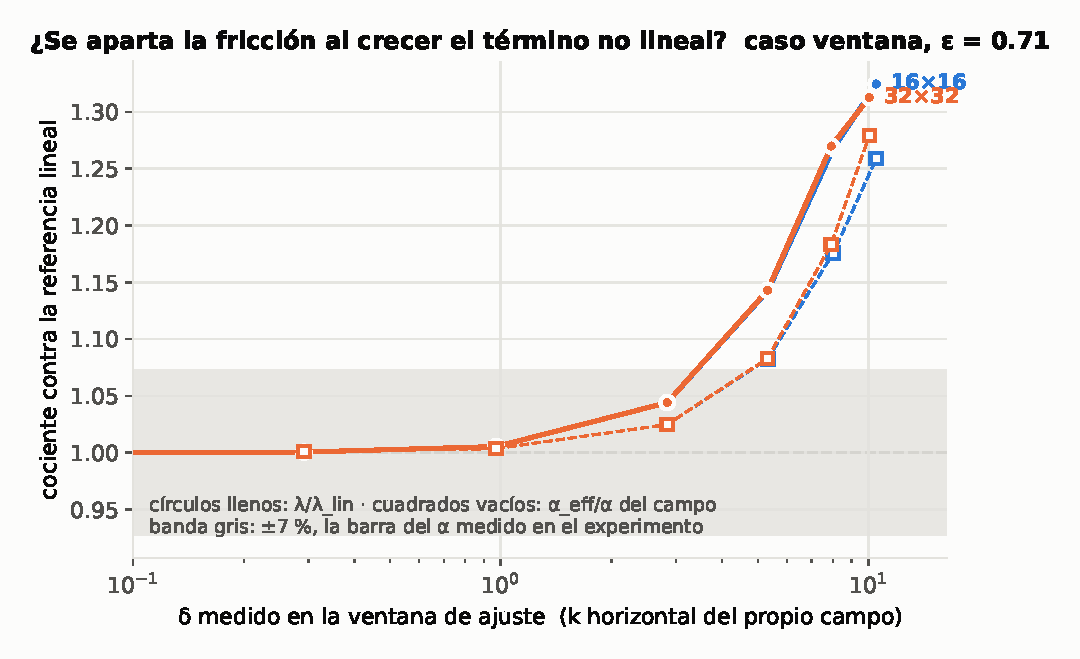
\includegraphics[width=.49\textwidth]{f7_barrido_delta_ventana.pdf}\hfill
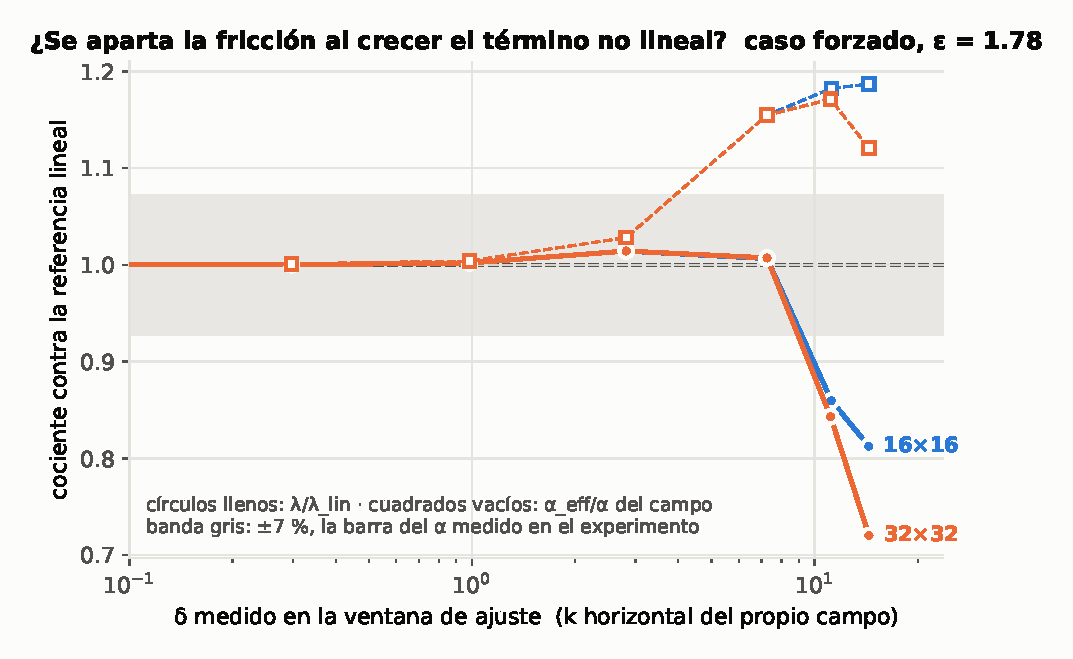
\includegraphics[width=.49\textwidth]{f7_barrido_delta_forzado.pdf}
\caption{Barrido en $\delta$ \etq{V-16}. Círculos: tasa sobre la lineal; cuadrados:
$\alpha_{\rm eff}/\alpha$; banda gris: la barra del $\alpha$ medido ($\pm7\%$). Izquierda,
$kh=0{,}71$ (la ventana del ajuste experimental); derecha, $kh=1{,}78$ (el fundamental de la
red de imanes).}
\label{fig:barrido}
\end{figure}

%=====================================================================
\section{Contraste con el experimento}
\label{sec:exp}

Se usaron cuatro decaimientos libres de la campaña de PIV del 02-06-25 (6 mm de KNO$_3$ al
$16\%$, 60 fps), reprocesados desde los TIF crudos con el $\Delta t$ óptimo del PIV
(figura~\ref{fig:exp}). El ajuste para $t>10$ s del ensemble da
\[
\alpha_{\rm medido}=0{,}0669\pm0{,}0049\ \mathrm{s^{-1}}\quad\text{contra}\quad
0{,}0685\ \text{(superficie libre)}\ \ \text{y}\ \ 0{,}274\ \text{(tapa rígida)} \etq{V-13}.
\]
Cualitativamente, la condición correcta es la superficie libre, no la tapa rígida que usan
hoy los códigos del grupo. Cuantitativamente queda una salvedad abierta \etq{P-02}. Para el
$k$ que el flujo sí tiene (59--130 m$^{-1}$), la tasa lineal $\lambda(k)$ es
0,072--0,085~s$^{-1}$, y el medido queda $7$--$22\%$ por debajo.

Lo que se descartó y lo que sí explica una parte:
\begin{itemize}
\item la no linealidad empuja al revés (§3);
\item el ajuste por anillos espectrales recupera $\nu k^2$ con el coeficiente correcto,
  $(1{,}03\pm0{,}10)\cdot10^{-6}\,\mathrm{m^2/s}$, y deja el déficit en la ordenada \etq{V-18};
\item un fondo de movimiento con la forma de la red de imanes, anterior al forzado, explica
  $4$--$5\%$ \etq{H-18}.
\end{itemize}
El acuerdo del $2{,}4\%$ con $\alpha_{\rm libre}$ no se presenta como acuerdo: el espesor
domina el error, porque medio milímetro mueve $\alpha$ un $17\%$.

\begin{figure}[h]
\centering
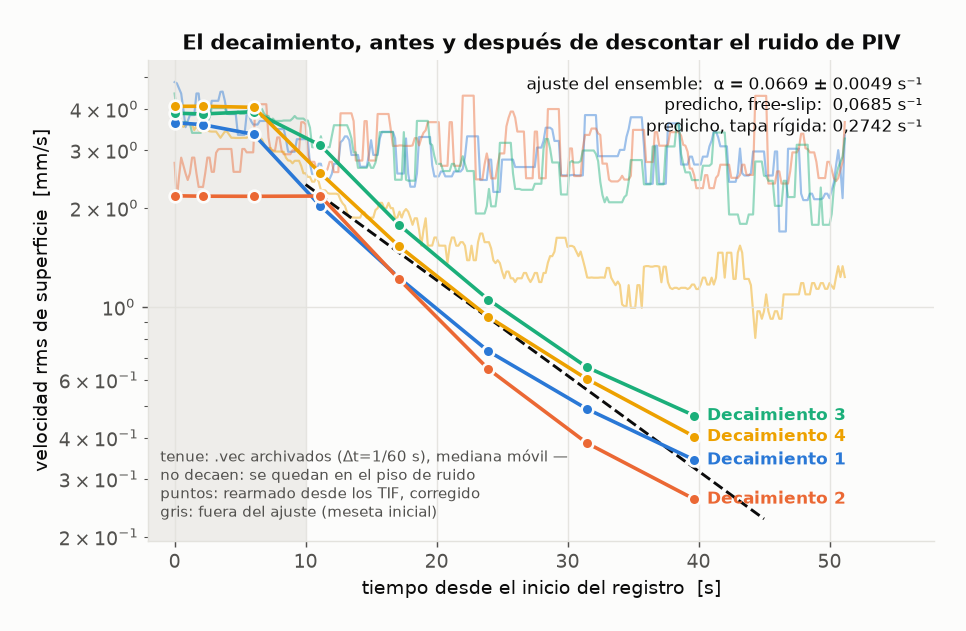
\includegraphics[width=.72\textwidth]{f1_decaimiento_claro.png}
\caption{El decaimiento medido \etq{V-13}. Trazo tenue: las series archivadas, con pares de
cuadros consecutivos, donde el ruido de PIV es del orden de la señal. Puntos y trazo grueso:
reprocesado desde los TIF crudos con $\Delta t$ óptimo; el decaimiento exponencial aparece
con $97{,}5\%$ de vectores válidos.}
\label{fig:exp}
\end{figure}

%=====================================================================
\section{La superficie deformable}
\label{sec:def}

\textbf{Lineal} \etq{D-49}. La presión pasa a ser Dirichlet en la superficie, y eso necesitó una
rama nueva del solver de Laplace y una proyección con una condición por cara. $\eta(x,y,t)$ se
integra como un campo propio, y la tensión tangencial, acoplada a $w$, se resuelve exacta.
Puerta 8/8.

El resultado que importa para la pregunta: a orden lineal, \textbf{el modo vortical del
experimento no siente la deformación} \etq{H-21}. Su efecto sobre $\alpha$ es
$O(\mathrm{Fr}^2)$, y eso justifica de manera cuantitativa el free-slip plano en la celda.

\textbf{Orden $N$} \etq{D-51}, \etq{D-52}. Las condiciones exactas de la superficie gráfica
se transfieren a $z=h$ por serie de Taylor en $\eta$, truncadas a orden $N=2,3$, con el
volumen de Navier--Stokes completo. $N=2$ tiene exactamente los términos del efecto
$O(\mathrm{Fr}^2)$.

Qué quedó verificado:
\begin{itemize}
\item el modelo es exacto contra la expansión de las condiciones de Wang, Tice y Kim
  (\href{https://doi.org/10.1007/s00205-013-0700-2}{ARMA 2014}), a $10^{-14}$;
\item en una onda estacionaria no lineal contra una referencia de geometría exacta, $N=3$
  tiene orden 3 (2,33 y 3,02) y $N=1$ orden 1;
\item un verificador independiente revisó el trabajo en dos rondas \etq{V-22}.
\end{itemize}

\begin{figure}[h]
\centering
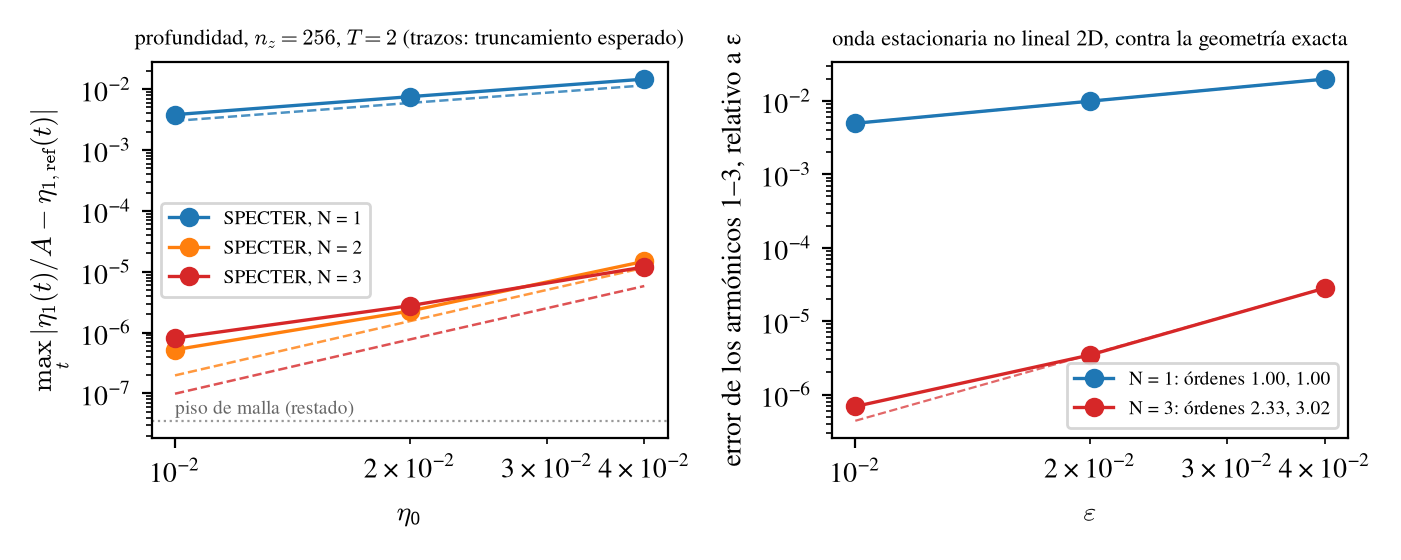
\includegraphics[width=.88\textwidth]{f_fs6_escaleras.png}
\caption{Verificación del orden $N$ (\texttt{numerico/fase6/escaleras.py}). Izquierda:
elevación media uniforme $\eta_0$, contra una referencia a profundidad $1+\eta_0$; los trazos
son el truncamiento esperado, en el que $N=2$ ya es $O(\eta_0^3)$ \etq{H-25}. Derecha: onda
estacionaria no lineal contra la geometría exacta; los trazos marcan las pendientes 1 y 3.}
\label{fig:esc}
\end{figure}

La puerta da 4/10. Los fallos corresponden a límites que encontró la implementación, no a
errores:
\begin{itemize}
\item $N=2$ está mal planteado donde $\eta<0$, por una capa espuria de espesor $|\eta|$ que
  crece como $\nu/\eta^2$ \etq{H-24}; el código aborta antes de ese régimen;
\item con elevación uniforme, $N=2$ ya es $O(\eta^3)$, así que un criterio estaba mal a
  priori \etq{H-25};
\item la tercera derivada espectral limita a $N=3$ \etq{H-26}.
\end{itemize}
En la celda nada de eso aplica, porque $\eta/\Delta z\sim10^{-3}$.

\textbf{A escala real} (figura~\ref{fig:sup}) se corrió la condición inicial de banda ancha de
\etq{V-19} con tope deformable de orden 2, a $g$ y $\sigma/\rho$ físicos, en $64^2$ y por 4
memorias (7,3~s), en el clúster: 2~h~24~min con 2 procesos. La laptop repite los primeros
2,7~s con 3 procesos, y el $\eta_{\rm rms}$ coincide a $10^{-13}$ relativo \etq{V-23}.
\begin{itemize}
\item La superficie, que arranca plana, se deforma con la forma del campo de presión del flujo
  vortical. $\eta_{\rm rms}$ baja \EtaRms{} mientras el flujo decae, con máximos de \EtaMax,
  y sigue a $U^2=\avg{u^2+v^2}$ en la superficie. Desde $t\approx1{,}2$~s, $U^2$ cae un
  factor $3{,}3$ y $g\,\eta_{\rm rms}/U^2$ queda entre $0{,}31$ y $0{,}42$.
\item El campo $\eta$ correlaciona \EtaCorr{} con la estimación cuasi-estática $p/\rho g$ hecha
  con la velocidad de superficie\propio. Encima quedan las ondas del arranque, débilmente
  amortiguadas.
\end{itemize}

\begin{figure}[h]
\centering
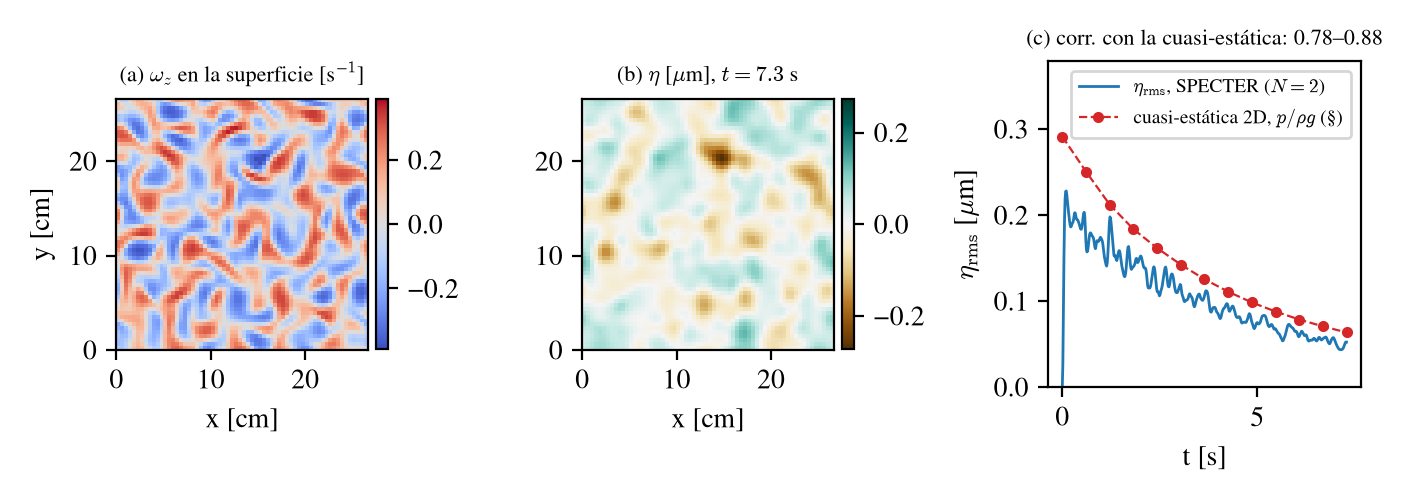
\includegraphics[width=\textwidth]{f_fs6_superficie.png}
\caption{Campos de superficie con la superficie deformable de orden 2 a la escala de la celda
(\texttt{numerico/fase6/campos\_superficie.py}, $64^2\times39$, 4 memorias, en el clúster).
(a)~Vorticidad en $z=h$ y (b)~elevación, en el último instante. (c)~$\eta_{\rm rms}(t)$, y
el nivel cuasi-estático estimado\propio{} con la presión 2D de la velocidad de superficie; el
título da la correlación entre los dos campos en los 12 instantes guardados.}
\label{fig:sup}
\end{figure}

%=====================================================================
\section{Salvedades y qué sigue}
\begin{itemize}
\item La viscosidad es la del agua, no la del electrolito; el espesor domina el error del
  contraste. \etq{P-02} sigue abierta.
\item El barrido en $\delta$ convergió en malla hasta $\delta\approx7$--$10$. La producción
  a la geometría real y la convergencia $64^2$ de \etq{V-19} están preparadas para el clúster.
\item El efecto $O(\mathrm{Fr}^2)$ de la deformación sobre $\alpha$ se calcula corriendo el
  mismo puente con \texttt{fsorder = 2} contra free-slip. Eso queda para el clúster.
\end{itemize}

\noindent\textbf{Repositorio.} El log de decisiones, hallazgos y verificaciones está en
\texttt{DECISIONES.md}; el estado y cómo retomar, en \texttt{ESTADO.md}. La versión extendida
del 17-09, con las derivaciones, es \texttt{informe/entrega.pdf}. El registro de la superficie
de orden $N$ es \texttt{numerico/fase6/REGISTRO\_fase6.md}.

\small\noindent Referencia principal: M.~Fontana, O.~P.~Bruno, P.~D.~Mininni y P.~Dmitruk,
Comput.\ Phys.\ Commun.\ \textbf{256}, 107482 (2020),
\href{https://doi.org/10.1016/j.cpc.2020.107482}{10.1016/j.cpc.2020.107482}. Las demás, con DOI
resuelto en Crossref, están en\\ \texttt{bibliografia/REFERENCIAS.md}. Un \propio{} marca una
estimación de esta sesión no validada contra bibliografía.
\end{document}
